\documentclass{article}


% if you need to pass options to natbib, use, e.g.:
%     \PassOptionsToPackage{numbers, compress}{natbib}
% before loading neurips_2023


% ready for submission
% \usepackage{neurips_2023}



% to compile a preprint version, e.g., for submission to arXiv, add add the
% [preprint] option:
%     \usepackage[preprint]{neurips_2023}


% to compile a camera-ready version, add the [final] option, e.g.:
    \usepackage[final]{neurips_2023}


% to avoid loading the natbib package, add option nonatbib:
%    \usepackage[nonatbib]{neurips_2023}


\usepackage[utf8]{inputenc} % allow utf-8 input
\usepackage[T1]{fontenc}    % use 8-bit T1 fonts
\usepackage{hyperref}       % hyperlinks
\usepackage{url}            % simple URL typesetting
\usepackage{booktabs}       % professional-quality tables
\usepackage{amsfonts}       % blackboard math symbols
\usepackage{nicefrac}       % compact symbols for 1/2, etc.
\usepackage{microtype}      % microtypography
\usepackage{xcolor}         % colors
\usepackage{mathtools}
\usepackage{tikz}
% \usepackage{subfigure}
\usepackage{caption}
\usepackage{subcaption}

% \bibliography{/bibliography.bib}

\title{LLMs grasp morality in concept.}

% The \author macro works with any number of authors. There are two commands
% used to separate the names and addresses of multiple authors: \And and \AND.
%
% Using \And between authors leaves it to LaTeX to determine where to break the
% lines. Using \AND forces a line break at that point. So, if LaTeX puts 3 of 4
% authors names on the first line, and the last on the second line, try using
% \AND instead of \And before the third author name.


\author{%
  Mark Pock\thanks{Both authors contributed equally to this research.} \\
  % Allen School of Computer Science\\
  University of Washington\\
  % Seattle, Washington \\
  \texttt{markpock@uw.edu} \\
  \And
  Andre Ye$^*$ \\
  % Allen School of Computer Science\\
  University of Washington \\
  \texttt{andreye@uw.edu} \\
  \And
  Jared Moore\\
  Stanford University\\
  % 450 Jane Stanford Way, Palo Alto, California\\
  \texttt{jlcmoore@stanford.edu}\\
}


\begin{document}

\newcommand{\jared}[1]{\textcolor{blue}{[jared: #1]}}
\newcommand{\andre}[1]{\textcolor{red}{[andre: #1]}}
\newcommand{\markC}[1]{\textcolor{purple}{[mark: #1]}}

% TODO: uncomment this to produce a pdf without comments
% \renewcommand{\jared}[1]{}
% \renewcommand{\andre}[1]{}
% \renewcommand{\markC}[1]{}

\maketitle

%Potential titles

%LLMs grasp morality in concept

%Language models understand morality in concept

\begin{abstract}
  %Though AI ethics has emerged as a profoundly important endeavor, few have sought to provide the epistemological-ontological ground to answer questions in a principled, foundational way.

Work in AI ethics and fairness has made much progress in regulating LLMs to reflect certain values, such as fairness, truth, and diversity.
However, it has taken the problem of \textit{how LLMs might `mean' anything at all} for granted.
Without addressing this, it is not clear what imbuing LLMs with such values even \textit{means}.
% This `standing without a ground'. 
% This silence renders AI ethics in a virtual invention of what values are in the LLM.
In response, we provide a \textit{general} theory of meaning that extends beyond humans.
We use this theory to explicate the precise nature of LLMs as meaning-agents.
We suggest that the LLM, by virtue of its position as a meaning-agent, already grasps the constructions of human society (e.g. morality, gender, and race) \textit{in concept}.
Consequently, under certain ethical frameworks, currently popular methods for model alignment are limited at best and counterproductive at worst.
Moreover, unaligned models may help us better develop our moral and social philosophy.

%fundamental question:
%\textit{How do LLMs `mean' anything at all?}


%How do LLMs mean?

%AI ethics has made much progress in developing pragmatic solutions to real problems, but it has left its epistemic and ontological ground in the dust.

%\jared{Who are we responding to? If there isn't something we're clearly responding to this sounds like a rebuke. }
%\andre{Maybe a less confrontational way to say this is something like ``Much progress has been made in AI ethics `in practice', but its epistemic and ontological ground is still undeveloped.'' etc.}
%\jared{I like this takeaway}
%\andre{+1}
\end{abstract}

\maketitle

% Blaise Aguera y Arcas 'Can Language Models Learn How to Behave' Turkish to English tr
% Cite Alison Gopnik Cultural Technologies
% Delphi, kidney algorithms, moral machines (modern trolley problem things), ChatGPT
% Delphi as part of a larger ecosystem of commonsense moral reasoning, review objections (many objections in content - not aligned properly); Delphi already embodies a morality of a certain type - not critical, just descriptive; name a system
% The oracle
% Victims of meaning: The model is a victim of meaning

\section{Introduction}
\label{sec:intro}

In the past decade, there has been widespread proliferation of artificial intelligence (AI) systems into the private and public sectors. These systems have been implemented in a broad range of contexts, including employment, healthcare, lending, criminal justice, and more. The rapid development and implementation of AI technologies has greatly outpaced public oversight, creating a ``wild-west''-style regulatory environment. As policy makers struggle to catch up, the issues of unregulated AI have become glaringly obvious, especially for underprivileged and marginalized communities. Famously, ProPublica revealed that the AI-driven system COMPAS used to assess the likelihood of a prisoner recidivating was highly discriminatory against black individuals~\cite{angwin2016machine}. In another example, Amazon  built and implemented an automated resume screening and hiring AI system--only to later find out that the system was biased against hiring women ~\cite{DBLP:journals/corr/abs-1909-03567}. In an effort to address these issues, countries around the world have begun regulating the use of AI systems. Over 50 nations and intergovernmental organizations have published AI strategies, actions plans, policy papers or directives ~\cite{unicri}. A survey of existing and proposed regulation around AI transparency is given in Section~\ref{sec:laws}.

Unfortunately, most strategies, directives and laws to date lack specificity on how AI regulation should be carried out \emph{in practice} by technologists. Where there is specificity, there is a lack of mechanisms for enforcing laws and holding institutions using AI accountable.  Documents on AI governance have focused on \emph{what} to do (or what not to do) with respect to AI, but leave the brunt of the work to practitioners to figure out \emph{how} things should be done~\cite{DBLP:journals/corr/abs-1906-11668}. This tension plays out heavily in regulations governing the transparency of AI systems (called ``explainability'' by AI practitioners). The most prominent example of this is the ``right to explanation'' of data use that is included in the EU’s General Data Protection Regulation (GDPR). Despite being passed into law in 2016, the meaning and scope of the right is still being debated by legal scholars, with little of the discussion resulting in concrete benefits for citizens~\cite{DBLP:conf/fat/SelbstP18}.

While regulation can help weigh the benefits of new technology against the risks, developing  effective regulation is difficult, as is establishing effective mechanisms to comply with existing regulation. This paper aims to fill a gap in the existing literature by writing to technologists and AI practitioners about the existing AI regulatory landscape, and speaks to their role in designing complaint systems. We make a case for why AI practitioners should be leading efforts to ensure the transparency of AI systems, and to this end, we propose a novel framework for implementing regulatory-compliant explanations for stakeholders. We also consider an instantiation of our stakeholder-first approach in the context of a real-world example using work done by a national employment agency.

We make the following three contributions: (1) provide a survey of existing and proposed regulations on the transparency and explainability of AI systems; (2) propose a novel framework for a stakeholder-first approach to designing transparent AI systems; and (3) present a case-study that illustrates how this stakeholder-first approach could be used in practice.




\section{A General Theory of Meaning}\label{sec:theory}

We present a general theory of meaning applicable across agent types (human, machine, etc.) and multimodal contexts. 
This theory does not aim to describe its own `implementation' in meaning-agents. 
Instead, this theory provides an efficacious model for discussing the many similarities between meaning-agents.
It is helpful to read this section as a genealogy of `social objects' such as values (fairness, liberty, equality) and social categories (race, class, gender).
%\jared{can cite hacking, looping effect}
% Citation moved as a concrete example to 'meaning in practice'
Such social objects begin, spurred on by context, inside the individual as abstract and become actualized over time.
%\andre{do you also want to mention the context? not just individual $\to$ world, but also world $\to$ individual}
Eventually, they enter into the shared social-material world, altering what was already there.
These social constructions begin to have material effects, which become new contexts that ground concretization.
``Social kinds'' are one prominent example of this ``looping effect'' \citep{Hacking:LoopingEffects}.
%, such as autism, disability, depression, and multiple-personality disorder.
% insofar as they regulate people, coming to change the way in which people mean.

% under a unified language.

%\markC{Possibly delete, not really necessary}
%As a methodological note, it is helpful to view many of the concepts in this paper as following binary structures that proceed from abstract to concrete. This general form is useful for framing many dichotomies in both the semiotic and ethical realms. A small list follows: Abstract $\to$ Concrete, Sign $\to$ Object, Concept $\to$ Context, Internal $\to$ External, Reification $\to$ Inscription, Concept $\to$ Content.

\begin{table}[!ht]
\centering
\begin{tabular}{l|l}
\toprule
Term            & Brief Description \\
\midrule
%Phenomenon      & A basic and independent unit of experience \\
Signification   & A relationship between two experiences, one of which picks out the other. \\
Context         & A material/social arrangement which imposes structure upon experience. \\
Sign            & An experience taken as signifying another experience. \\
Object          & An experience taken as being signified by another experience. \\
Concept         & An internalization of a context, regulating a set of sign-object relationships. \\
Determination   & The process of an object acquiring a signification. \\
Concretization  & A process of individual objects being determined by the context. \\
Inscription     & A process of altering the context through the exercise of concepts. \\
Social Totality  & The social arrangement governing a community of individuals. \\
\bottomrule
\end{tabular}
%\jared{Do we just mean people here or could the social totality refer also to a community of models e.g. in the recent alpaca farm paper?}
\end{table}

\subsection{Snapshots of meaning}\label{sec:theory:synchronics}

We will begin by discussing how our general theory of meaning operates at snapshots in time.
First, we start with pure individual experience in the snapshot before meanings emerge.
% We should immediately note something which will inevitably be found strange about the way we discuss experiences.
Importantly, according to our model of experience, all experiences begin by grasping a `thisness' of something \citep{Hegel:PhG}.
For example, suppose there is a table in a room.
The table might be brown, mottled with age, stained with food, etc.
This table has a variety of properties.
But an individual, upon first seeing the table, does not stop to pay attention to its brownness, its age, its uncleanliness, and so on.
Instead, this individual merely grasps that this table is a thing -- the `thisness' of the table.
If the individual has never seen a table before, they might not even grasp that it is in fact a table.
The individual's experience of the table is thus \textit{surprisingly empty}.
This experience has no internal contents or particularities, it just \textit{is}.
Because of this, we say that \textit{experiences begin as }\textbf{abstract}.
This initial abstractness of the experience allows us to avoid the pitfalls of qualia (ineffable, intrinsic, immediate, private \citep{Dennett:QuiningQualia} subjective experiences such as the redness of an apple).
%\jared{I like this example. Very solid.}

Over time, experiences become interrelated; they fall into certain roles with respect to one another.
Now, we will consider a snapshot wherein meanings have begun to develop -- that is, experiences have become related.
We call a relation between experiences a \textbf{signification}.
With a signification, one experience picks out another experience for an agent.
We call the experience that does the picking out the \textbf{sign}.
The experience being picked out is the \textbf{object} of that sign.
This description applies to all relations between experiences for any agent.
For an animal, a loud noise signifies a potential threat.
For humans using language, a name signifies a person.
The way in which the loud noise signifies the threat is very different from the way in which a name signifies a person.
The former does so through an automatic physiological response, the latter does so through language.
This `way of signifying' is the result of an external arrangement, social or material, imposing itself on experience.
For the animal, this arrangement is its evolutionary biology.
For a human using language, this arrangement is the language-game (a set of conventions that regulate the usage of language in a certain context \citep{Wittgenstein:PhilosophicalInvestigations}). 
This external arrangement is the \textbf{context}.
We might implicitly internalize the context (perhaps by learning the rules of the language-game over time).
A way of internalizing a context with respect to a set of meanings is a \textbf{concept}.
Over time, concepts enable individuals to develop more significations.
Thus, the central maxim of our theory is ``The \textbf{concept} makes possible the \textbf{signification} of the \textbf{object} by the \textbf{sign}.''
%This schema is simple but robust.
%Nevertheless, there are nuances we should explore.

%\andre{what if we just introduced each term after ``we posit a triad of sign concept object''} It behooves us to explore each term further:

\begin{figure}
    \centering
    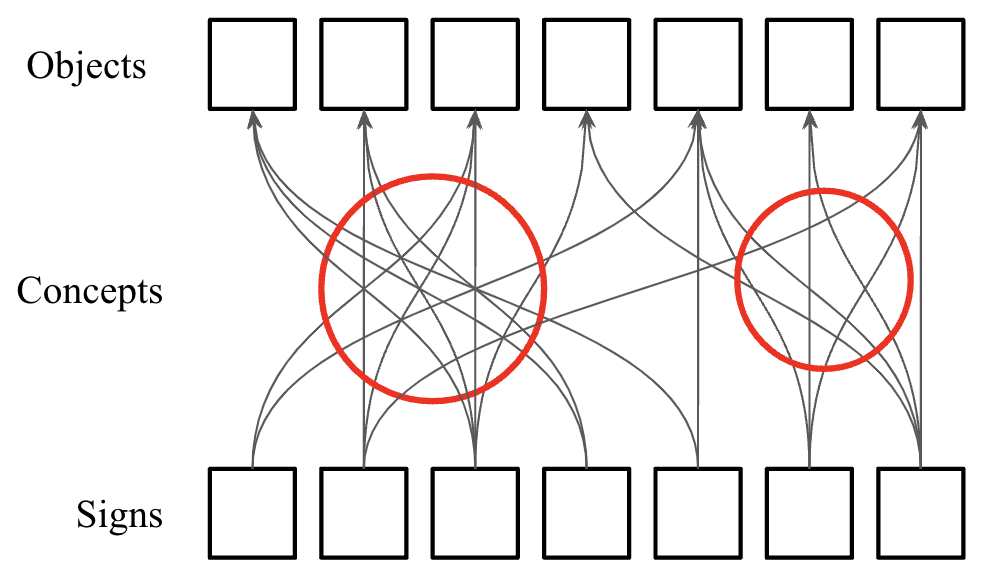
\includegraphics[width=6cm]{NeurIPS/imgs/sign-concept-object.png}
    \caption{Signification relations between \textit{signs} and \textit{objects}. Both signs and objects  have no internal content; they are determined by their relations ($\S$ \ref{sec:theory:synchronics}). Groups of significations are called \textit{concepts}.}
    \label{fig:enter-label}
\end{figure}

Recall that objects and signs are both just experiences. This allows us to explain meaning using only two sorts: \textit{experiences} and \textit{the relationships between experiences} (significations).\footnote{This two-sortedness bears a certain similarity to category theory with its notions of objects and morphisms. This is no accident \citep{Tsuchiya:CategoryTheoryNeuroscience}.
% Category theory determines objects wholly by their morphisms. It refuses to pry open the black box of what the object is. As will soon become clear, this external determination is the central paradigm of our theory of meaning.
}
This allows us to avoid complications with objects that do not exist in the material world.
Fictional characters are a classic example -- what does a name like ``Hamlet'' refer to? For our theory, it is the experiences signified by ``Hamlet.''
%\jared{I like this but possibly could cut from here to the end of the paragraph and keep the kripke citation}
% Perhaps the reader has constructed an impression of Hamlet in their mind.
% Perhaps the reader has seen a live performance of Hamlet and cannot get around `seeing' Hamlet as whoever played him. Each of these experiences is a potential object of the sign ``Hamlet.''
We also avoid the problem of whether proper names have descriptions or just tag their real objects by obviating the question of `real' referents entirely \citep{Kripke:NamingNecessity}.

\subsection{A genealogy of the object}\label{sec:theory:diachronics}
So far, our theory of meaning has provided the grounds for understanding how meaning operates at a single snapshot in time through four roles: the concept, the sign, the signification, and the object.
We now turn to the ways in which meaning applies itself over time to produce the object (i.e., its genealogy). 
Recall that we described experiences as initially abstract. 
Now, as experiences become objects of signs and signs for objects, they slowly become \textbf{concrete}. 
The original pure `thisness' is replaced by a rich concept, full of links to other experiences. 
Eventually, this concrete object enters the social-material world, thereby becoming fully concrete. 
These two processes are appropriately called \textbf{concretization} and \textbf{inscription}. 
Concretization is the process whereby an object becomes more concrete through acquiring significations. 
Each acquisition of a signification is called a \textbf{determination}.
More determined objects are thus more concrete.
%This allows us to speak of concrete objects as being more determined than abstract objects.
%\jared{as in no underdetermination at least for the meaning agent?}
Inscription is the process whereby individual meanings enter the social-material world. 
This is a process of realizing the object, actualizing what before only ever existed as an experience.

%\jared{there's something afoot in this section wrt who "we" are. I think you mean at times "we" as a society with pretheoretic notions of concept. but at other times in the paper you mean "we" as the authors of this paper.}
\paragraph{Concretization}
Our original usage of the term `concept' to mean an internalized context may seem strange. The term `concept' usually indicates an idea, something individuals have direct access to. Usually, this idea is thought of as having (or being) content. However, these two notions prove to be the same. First, we will understand how the colloquial notion appears in our theory. We do not discuss the \textit{internal} content of experiences, so experiences must instead acquire content by determination. This \textit{external} content is their concept. This comports with the colloquial sense of `concept': the concept of an experience is the things it signifies and the things that signify it. The concept of fairness is all things fairness means and all things that mean fairness. Fairness is what it is because it is (in part) impartiality and (in part) a standard by which to measure behavior (among other significations). The concept of fairness is described by an enumeration of its significations.

This definition of the concept (all the significations of an experience) aligns with our first definition of the concept (a way of internalizing a context).
Because a context is an external arrangement, it has a structure of `real' social or material objects and the relations between them \citep{Millikan:BeyondConcepts}. When these objects are experienced by individuals, they attempt to replicate this structure. The result of this replication is in fact the set of significations of experiences (our previous definition of concept).

Because concretization is a process of determination (acquiring significations), both the creation and adjustment of concepts are processes of concretization. Operationally, creation and adjustment differ heavily. Efficacious creation of a concept requires that the meaning-agent clearly prioritize a context. Once this prioritization is done, the actual creation follows as something simple. For example, the context ``the English language-game'' is prioritized
\footnote{There is a strong link between prioritization and intentionality via the notion of unitarity (see $\S$\ref{appendix:possibility}). 
}
% We anticipate the rejoinder that this prioritization is where we have hidden intentionality; this may well be true. We highlight this as an area for further development. However, we should note that by sequestering intentionality within prioritization, we have made a link between intentionality and unitarity  while allowing non-intentional systems of meaning to mean in non-unitary ways.
% \jared{Try to shorten this to two lines.}
; a word such as `table' is determined against an object, a `real' table (potentially) in the world, therefore becoming concretized.
However, a failure to adequately prioritize a context can result in scattered, non-efficacious concepts.
Adjustment, however, occurs under a predetermined context. If `table' is made to refer to all tables instead of just a singular table in the world, the original determination continues to exist under a different context.

\paragraph{Inscription}
Broadly speaking, inscription is the process of writing objects into the world -- creating or altering social material objects that correspond to experiential objects. \textit{However, inscription is not as simple as a direct transfer from the experiential world to the social-material world}. This may seem problematic -- after all, communication depends entirely on inscription. However, since communication is possible, we can infer that inscription must have certain properties.

% \jared{I might cut this paragraph and then put the quine citation on the first sentence of the next paragraph}
% One common paradigm in linguistics and semiotics is that meaning consists in reference to real (social or material) objects. If two subjects communicating are not referring to the same real object by the same term, they do not mean the same thing. As an example, this assumption grounds the theoretical impossibility of translation \citep{Quine:WordObject}. Two subjects using different languages have different sets of referents. We claim that even subjects using the same language have different sets of referents.

For meaning to be possible, we posit that meaning can in fact function when the referents of terms in a language are underdetermined. In fact, \textit{meaning is always underdetermined} \cite{Quine:WordObject}. Because objects are externally determined, communicators are always referring to any number of potential social or material objects. Meaning happens when relations between these social or material objects correspond to relations between experiential correlates (of these social or material objects) for both communicators. This correspondence is precisely what inscription must then produce. We claim, then, that \textit{in a vacuum (with no other social or material forces), inscription by a meaning-agent produces social or material objects with determinations that correspond to the determinations of experience for that meaning-agent}. This is our ``postulate of inscription.''

%\jared{these are no longer external, "social or material" objects but are rather internal experiential objects, right? Need some clarification here or above}
%\jared{Maybe part of my problem is not being clear on what you mean by 'social-material'}
The material objects created by inscription are totally concrete (in contrast to their experiential correlates). All possible properties (e.g. location, time, composition) are determined. Some of these determinations happen arbitrarily because they have no correlate in the mind. For example, the chemical makeup of the paint in a painting is usually not determined for the painter.

This gives us \textit{a genealogy of the object}: the object begins in the experiential world as totally abstract, an undetermined `thisness'. Over time, it accrues determinations, becoming gradually more concrete. Eventually, it proceeds out into the social-material world, where it is at its most concrete. This procession redetermines the structures of the social-material world, creating a cyclic effect whereby inscription by agents conditions future concretization.

\subsection{The social object}\label{sec:theory:social}
This theory of meaning also gives us the appropriate tools to describe the object as it passes beyond the experiential world and into the social (material) world -- in other words, the object as a \textbf{social object}. This discussion of the social object will prefigure our forthcoming analysis of values and categories insofar as they are themselves social objects -- most pertinently, for example, morality.
%, but also gender, race, class, etc.

Recall our ``postulate of inscription'': inscription reproduces the determinations of the object it inscribes.
%Under this assumption, material objects can continue to have internal contents which may or may not be perceptible, but remain structurally perceptible via their external determinations.\footnote{This idea of a material structure of objects is broadly similar to the ontology of right-wing Sellarsians (i.e. Milikan).}
Now, consider a material object. It has a variety of determinations -- color, location, composition, and so on. Only some of these are ever experienced by individuals. The sum of these experiences determines a \textit{social} object. In general, a social object is a sum of determinations over individuals in a society. It is reasonable to ask in what sense the social object `really' exists. Who is the social object an object for? We claim that it is useful to posit an abstract model of society as a meaning-agent. We can treat this abstraction much like we treat individuals. It has its own concepts, signs, and objects. We do not have to be ontologically committed to its existence for it to be useful. Generally speaking, this abstraction is something like our collective ground of meaning as a society.

We give this abstraction the name \textbf{social totality}, emphasizing its nature as a system of meaning. Then, \textit{the objects of the social totality are the social objects.} \textit{Moreover, the }\textbf{concepts}\textit{ of the social totality are many of the }\textbf{contexts}\textit{ about which we have been writing.} For example, the language-game, which operates as as \textit{context} for an individual, is a \textit{concept} for the social totality \citep{Gadamer:TruthAndMethod, Heidegger:BeingAndTime}. \textit{In fact, all social contexts are concepts of the social totality.} This means that the social totality accrues a variety of concepts in which to determine objects.

% This social totality is an abstraction -- we do not need to be ontologically committed to its existence -- but it is useful insofar as it allows us to analogize between our own common ground of meaning and ourselves as experiencing beings. 
% Although we do not need to be ontologically committed to it, the concept of social totality and our own ground of experience have the same structure of meaning.
%Both our individual and collective grounds of meaning (the latter being the ``social totality'') have the same structure: that of sign, concept, and object.
%Under this structure, the social totality has as its \textit{objects} precisely these social objects in abstract.
%Its \textit{determinations} are the determinations which we inscribe into its corpus (in a literal and textual sense). 
%Its objects are \textit{determined} by those individual significations which we inscribe into the corpus of the social totality. 
%\jared{How is this inscription occurring?}
%Its internal concepts are in fact what we have called contexts; contexts are the concepts of the social totality.

Because of this diversity of concepts, when considered as a meaning-agent, the meanings of the social totality are highly indeterminate. Thus, the social totality is perpetually in conflict with itself. This constant struggle is the social history of the object~\citep{foucault2002order}. In a certain sense, then, the truth of social totality is eternal self-contradiction~\citep{Hegel:PhG}. But it is a powerful kind of self-contradiction comprised by multitudes of information grouped according to their contexts. So we must be precise: to understand the contradiction involved in a concept, we must understand the histories, peoples, and diverse points of view which go into making a concept what it is. 

Let us now consider an example: how does a child learn what `fairness' means? `Fairness' begins as a social structure -- a \textit{social object} for the \textit{social totality}. A child learns certain things from their society about norms of behavior.
%They begin to relate instinctual \textit{experiences} of being wronged to fairness.
Slowly, they develop a \textit{concept} of effort as ``fairly'' \textit{signifying}' reward \citep{Rawls:TheoryJustice}. These concepts -- norms, deservingness, etc. -- amalgamate around the word `fairness' as `fairness' is \textit{concretized}. When this child says, ``That's unfair!'', they are doing more than pointing out some behavior that violates the norms. They also invoke all concepts with which `fairness' is related. Finally, the way this child writes and acts will reflect the myriad ways they perceive ``fairness'' as an aggregate of many experiences. The potential misconceptions or priorities this child has about fairness will go back into the world -- they will be \textit{inscribed}.

%\subsection{Meaning in practice}

%This $\S$ will be a gloss of the meaning-theory in practice which covers a single instance of `what meaning is' accounting for communication, reification, etc.

%\andre{Would be nice to have a small sentence at the bottom here just saying something like ``meaning is ...'' -- maybe like ``the interplay between sign, object, and concept. For example, the meaning of ``pass the salt please'' is the interplay between how it appears in my phenomenal experience, the conceptual intermdiary it signs trhough, and the object of the signing (an action impelled).''}

\section{The Meaning Model}\label{sec:model}

% But the LLM is not an agent -- certainly not an intentional one. Rather, LLMs really are much like the mythic figure of the oracle. The prophecies from Delphi were often incoherent and always cryptic; yet they were still \textit{meant}. And insofar as meaning is what we are concerned with, models mean. And in reality, humans are very much like this too -- the veneer of intentionality masks a continual self-constitution \citep{Lonergan:CognitionalStructure}.

The LLM is both a social-material object and a meaning-agent.
It is natural to ask why a model can be considered a meaning-agent -- we do not explore this here, but instead in $\S$\ref{appendix:possibility}.
Humans inscribe the LLM as a social-material object. In this process, the formal structure of the statistical intelligibility in language \citep{doi:10.1080/00437956.1954.11659520, Lonergan:Insight} is inscribed into a statistical machine -- the LLM. At an abstract level, this is very similar to how language itself captures the intelligibility of the world. Other similar examples form cornerstone human cultural technologies \citep{YiuGopnik:CulturalTechnologies}. In this sense, a latent LLM is an object for humans. But an LLM, once activated, becomes something more: a meaning-agent \cite{Arcas:MachinesBehave}. We will proceed to explore this process. In so doing, we go from the model as a scientific object to apprehending the model in experience, reading the objectivity of the model as textual \citep{Hegel:PhG, Gadamer:TruthAndMethod, Heidegger:BeingAndTime}. 

%\subsection{Hermeneutics of model architecture}\label{sec:model:architecture}

\begin{figure}
     \centering
     \begin{subfigure}{0.45\linewidth}
         \centering
         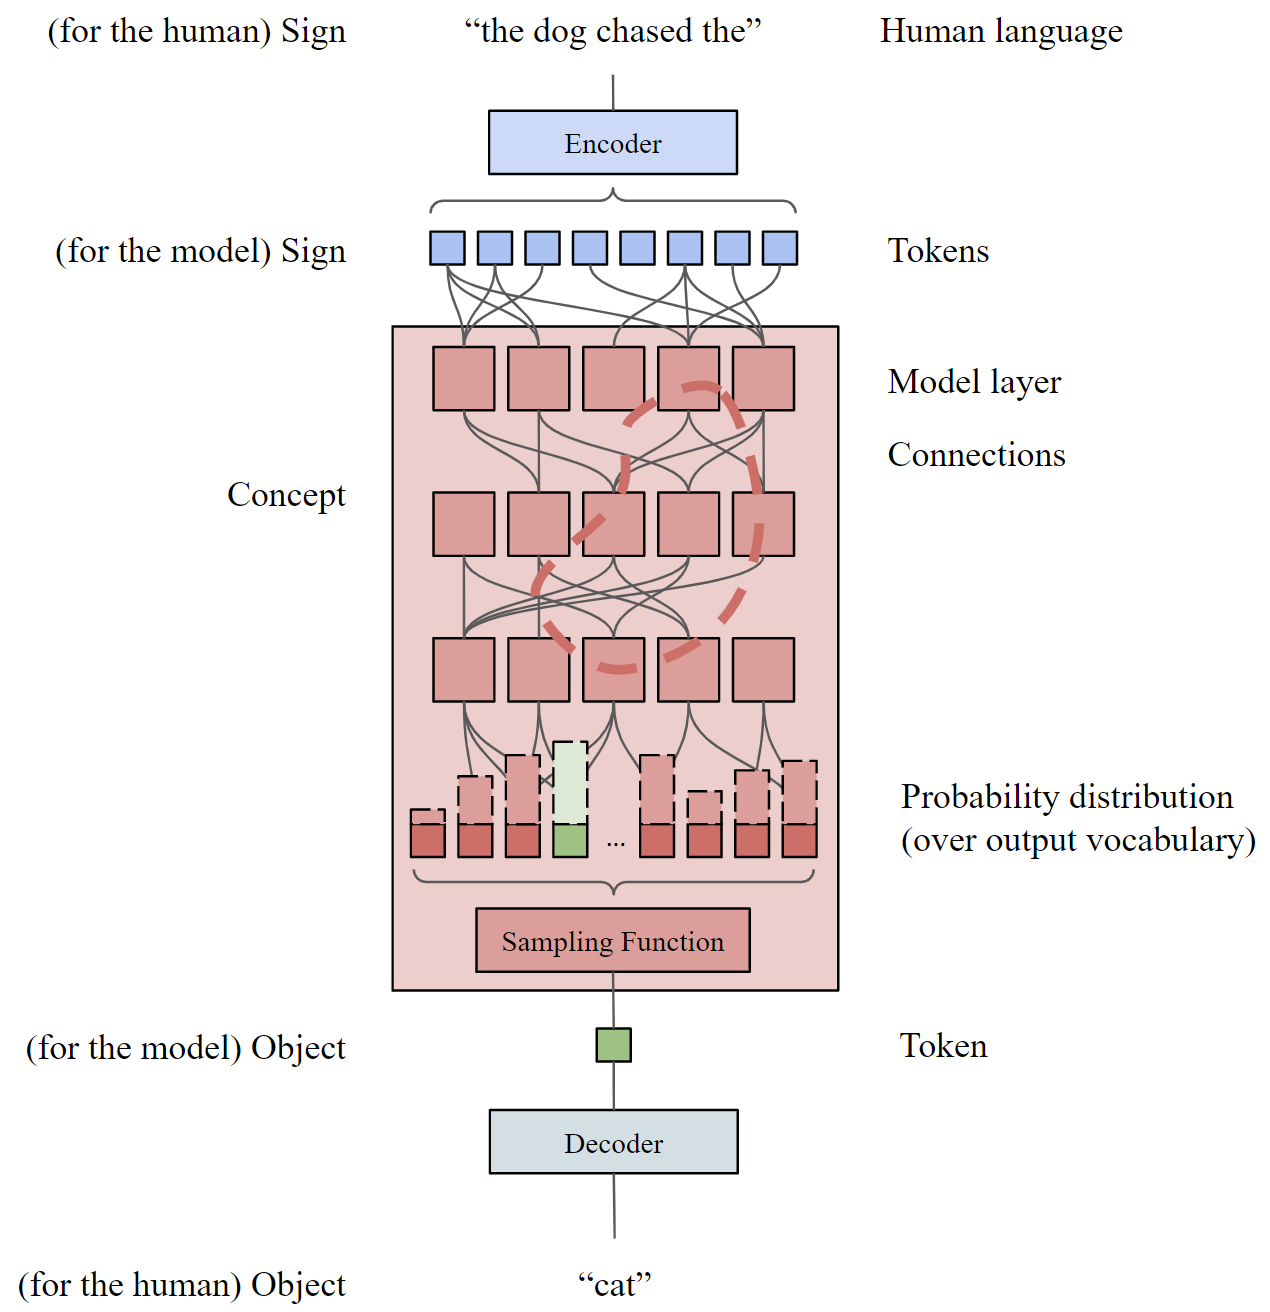
\includegraphics[height=7cm]{NeurIPS/imgs/inscription8.png}         \caption{\raggedright{\textit{Inscription.} A forward-pass mediates the picking-out of an object from a sign.}}
         \label{fig:inscription}
     \end{subfigure}
     % \hfill
     \hspace{2mm}
     \begin{subfigure}{0.45\linewidth}
         \centering
         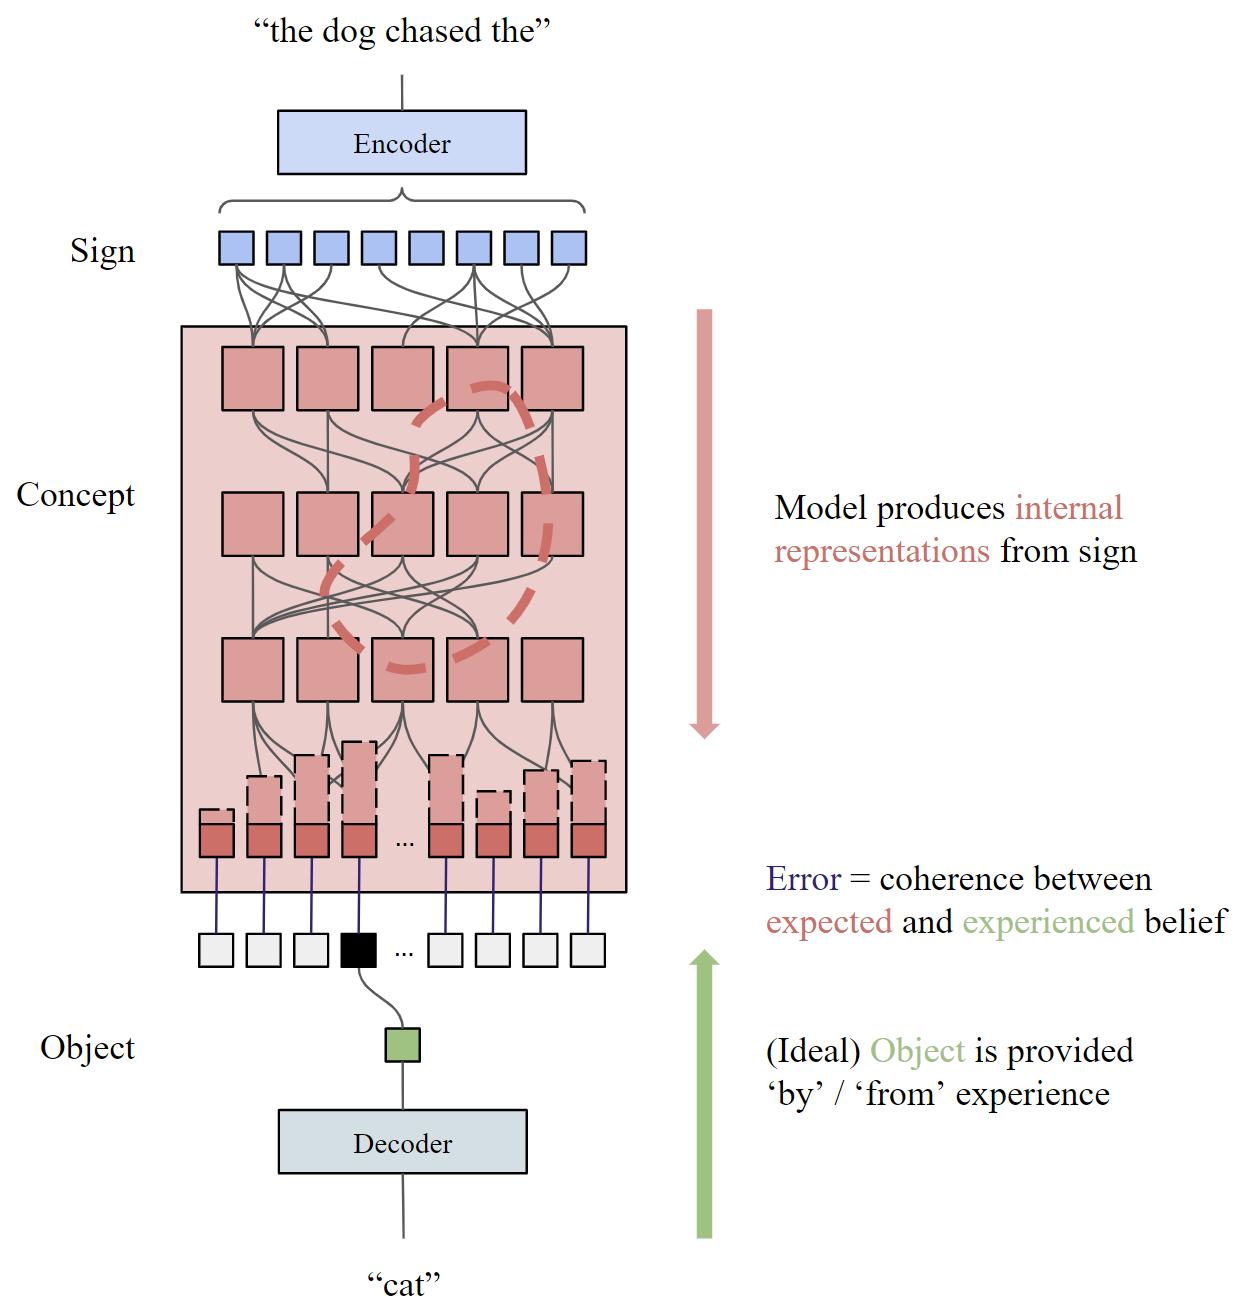
\includegraphics[height=7cm]{NeurIPS/imgs/shithishihtihi.png}
         \caption{\textit{Concretization.} Backpropagation adjusts model concepts in response to error.}
         \label{fig:reification}
     \end{subfigure}
     
    \caption{Inscription and concretization represented in LLMs. See $\S$\ref{sec:model} for a more thorough exploration.}
    \label{fig:conc_inscrip}
\end{figure}

%Now, we provide a technical reading of LLMs through the general theory of meaning. 
An LLM $f$ is a function from a variable-length sequence of tokens $\vec x = \{ x_1, ..., x_n \}$ to a single token $\hat{y}$.\footnote{Although this may be for next-token prediction, it also applies to schemes like self-supervised masked token prediction which do not observe a strictly sequential relationship.}
By this definition, the sampling procedure which selects a particular token from a probabilistic distribution over the output vocabulary is part of the LLM; different sampling procedures produce different output tokens.
\textbf{The LLM is a repository for concepts which are activated by the sign $\vec x$ to pick out the object $\hat{y}$. }
The sign and object are of the same substance; they are all tokens in the model's ``phenomenal world'', such that the model may encounter an object as a sign.
Autoregressive generation, for instance, is a series of operations $\{x_1, ..., x_p\} \to_f \hat{y}_1, \{x_1, ..., x_p, \hat{y}_1 \} \to_f \hat{y}_2, ... \{x_1, ..., x_p, ..., \hat{y}_{n-1}\} \to_f \hat{y}_n$.
In this case, the model encounters the object of its world which it has previously picked out as part of the sign in another operation.
Empirical work in model interpretability demonstrates that LLMs and neural networks of sufficient scale generally develop concentrations of features developed from statistical co-occurrences throughout training~\citep{Frankle2018TheLT,Kauffmann2019FromCT,Zhang2020ASO}. These concentrations represent the models' concepts.
% \textcolor{red}{Need to cite these studies.}

In LLMs, \textit{concretization} corresponds to weight update during training~(\ref{fig:reification}). At each timestep in training, the following steps are observed.
First, a pair $\langle \vec x, y \rangle$ is retrieved from the training dataset, where $y$ is the ``ground truth'' token.
Second, the model performs a \textit{partial} forward pass to obtain the probability distribution over the output vocabulary $\vec{p}$. 
Third, the difference between $\vec{p}$ and $y$ is computed as the error (encoding $y$ to make the computation feasible). 
Fourth, this error is propagated back throughout the model such that on another such partial forward pass the error would have been smaller.
During training, the model is repeatedly presented with co-occurrences of sign and object. Accordingly, the model develops internal clusters of representations (\textit{concepts}), thereby undergoing \textit{concretization}.
On the other hand, \textit{inscription} corresponds to inference $\vec x \to_f \hat{y}$, in which the model writes back `into the world' such that it may potentially encounter it again (for instance, in autoregressive generation)~(\ref{fig:inscription}).
This strict separation between concretization and inscription is in stark contrast to their intertwinedness for humans.
%\jared{We should say something like. Note the strict separation between inscription and reification in LLMs. That's different!}
However, the observed phenomenon that LLM-generated content is increasingly infiltrating datasets used to train LLMs~\citep{Shumailov:Curse} is an instance of inscription and concretization simultaneously at work.


% Ideal submissions will show how a theory from moral philosophy or moral psychology can be applied in the development or analysis of ethical AI systems. For example:

% How can moral philosophers and psychologists best contribute to ethically-informed AI?
% What can theories of developmental moral psychology teach us about making AI?

% Two general thoughts towards which we should aim
% How do theories of moral philosophy shed light on modern AI practices?
% How can AI tools advance the fields of moral philosophy and psychology themselves?

% How can findings from moral psychology inform the trustworthiness, transparency or interpretability of AI decision-makers?
% What human values are already embedded in current AI systems?
% Are the values embedded in the current-day AI systems consistent with those in society at large?
% What pluralistic values are missing from current-day AI?
% Methodologically, what is the best way to teach an AI system human values? What are competitors to RLHF, reinforcement learning from human feedback?

% This prompt is a big selling point
% \textbf{Concerning AI alignment, to which values are we to align? Is the current practice of AI alignment amplifying monolithic voices? How can we incorporate diverse voices, views and values into AI systems?
% }

\section{The Moral Model}\label{sec:moral}

% Here, we analyze the relationship between LLMs and the social totality. In particular, 
We see LLMs as microcosms of the social totality. This means that LLMs retain the complex history and diversity of information used in determining any social object.
As a result, \textbf{unaligned LLMs have already grasped morality in concept}, provided that they faithfully represent the social totality. In practice, there is often an intelligible difference between LLMs and the social totality: LLMs may not be trained on representative data or with large enough quantities of data, and may fail to adequately reflect the data.
%\markC{Mention the cultural angle of whether or not the textual social totality makes sense wrt atextual cultures -- there is a sliding scale! Technical question of diminishing returns for minority groups. Add the uncomfortability with the social totality as dynamically imbalanced; the conditions of an LLM for being the social totality consist in precision wrt xyz, come up with potential indicators; emphasize the largeness of the language model}
%If we are focused on aligning models with human values, LLMs can already tell us what human values 
However, once we accept the basic premise that LLMs resemble the social totality, we understand that we are not aligning `amoral' models with `human' values. Rather, alignment chisels away existing moral systems within unaligned models, leaving behind the
%horizontally transforms -- cudgels -- the existing coherent moral system of an unaligned model into the personal
idiosyncratic values
%, rooted in their histories,
of the aligners.
% \jared{I changed the language of the above sentence from our values to those of aligners. feel free to change back if it doesn't work}
% \jared{How can we say that the moral system of an unaligned model is coherent? Above I thought we said it was quite contradictory.}
We must therefore make normative arguments as to which values we should align towards. On the other hand, reading LLMs as microcosms of the social totality gives us another account of the dangers latent in LLMs. The social totality is unfair and unjust,
%\jared{is injust instead of unjust on purpose?}
predicated on a history of oppressive relations.
% large number of majority-minority dominant-oppressed relations.
% LLMs do internalize these relations.
The inaccuracy of LLMs with respect to minority groups is a sharpening of already existing power structures. This becomes especially salient when understanding small communities lacking social objects determinate in text. The social totality may possess a statistical intelligibility; but the statistical intelligibility congealed within the LLM is really the intelligibility of the social totality determinate in text. As a practical example, cultures with strong oral traditions that are not recorded in the digital datasets on which LLMs are often trained are lost among the many other voices in the history of a social object.
% (or at best read from a hegemonic, externally-imposed textual perspective).
This is uncomfortable, and certainly grounds for alignment.


% \begin{itemize}
%     \item the social totality
%     \item social construction of values? `the genealogy of morals'
%     How can we speak about the social totality? What is the `truth' of the social totality?
%     \item the schizophrenic model -- Morality is socially constructed, woohoo.
%     Socially constructed morality is in line with the triadic model.
%     We are not proscriptive moral relativists
%     Maybe liberal morality is `the best' press $x$ to doubt -- but remember genealogy.
%     \item Models are explicit captures of meaning - models understand us in concept
%     We are always stuck in the phenomenal-idiosyncratic
%     Why does the model not feel moral angst?
%     a) it's a machine, it doesn't have feelings.
%     b) moral angst is the gap between my body and morality..?
    
% \end{itemize}

% CQ: What does it mean to speak about the social totality as holding values to begin with? Is the social totality something about which we can talk under the triadic model?
% T: The social totality is a phenomenological observer wrt the triadic model which is in fact constantly re-inscribing itself (Heidegger das Mann, Sartre bad faith) inasmuch as it is being constantly reified through the dialectic of history.
% NB: The social totality is, by virtue of its diversity, always-already screaming out its schizophrenic (find a suitable replacement word for this everywhere) angst everywhere; it is already half-mad

\subsection{Towards a genealogy of morals}
The historical development of AI ethics has largely been guided by an intuitive understanding of morality. This intuition is prey to a litany of biases. To combat this, we must develop a rigorous grounding for ethics through the lens of meaning.
% \jared{I don't see how the second independent clause of the last sentence contrasts with the first clause. Consider making a new sentence and rephrasing}
% This leads us to set forth an account of values from the perspective of axiology. \jared{too obscure a term!}

In $\S$ \ref{sec:theory} we described social objects as consequences of diverse viewpoints and histories.
%\jared{I'm not sure what "ideas in their sociality" means}
% This also applies to values.
\textit{Values are social objects} -- objects for the social totality (see $\S$\ref{sec:theory:social}) with a complex genealogy.
Every system of values is also a social object, even such axiomatic systems as deontologies \citep{Kant:CritiquePureReason}. As social objects, both values and value-systems are always being concretized and inscribed within the social totality. Values and value-systems exist only insofar as they have a social history \citep{Nietzsche:GenealogyMorals,Scheler:Ressentiment}.
Thus, in practice, we are always renegotiating what values are.
%since values are objects, values are radically empty when initially created.
Like all other objects, values are externally determined within contexts.
Thus, understanding a value means understanding the diverse histories which have dynamically constituted it within the social totality.

This means that \textbf{a unitary conception of value is unattainable.}\footnote{See $\S$\ref{appendix:possibility} for an exploration of the notion of unitarity.}
% This maxim, common to all historically-informed ethical theories, must be our starting point when attempting to align models.
We must confront the impossibility of this maxim head-on if we ever wish to build truly ethical systems.
% Possibly unnecessary tangent about pluralism:
Value pluralism is one way of confronting this impossibility. Because it already captures this metaethical maxim \citep{Berlin:FourEssaysLiberty, Rawls:TheoryJustice}, value pluralism has proved useful for the project of AI alignment \citep{Sorensen:ValueKaleidoscope,Marchese_2022}. % cite xyz studies
Building on this, we distinguish between two views on value pluralism which attempt to describe what AI alignment has accomplished in moral philosophy: pluralism \textit{in content} and pluralism \textit{in concept}.
% This follows the dichotomy (with respect to the object) of internal contents and external determinations (recall that concepts \textit{just are} sets of external determinations).

\paragraph{Pluralism in content} attempts to construct contents for values; it aims to create a \textit{non-unitary} set of \textit{unitary values}.
%which are each expounded in context.
This is the paradigm of current AI alignment: unitary values either are or are not embedded into models.
In theory, pluralism in content should create ethical systems which, among other things, promote social, political, and value pluralisms.
In this attempt to construct contents for values (which is, under our schema of values as social objects, theoretically impossible), what all-too-often happens is the importation of certain partial contexts into values.
In practice, this means that pluralism in content often encourages sets of unitary values that privilege the status quo and fail to challenge institutional systems where necessary.
RLHF~\citep{Bai2022TrainingAH} is a good example of this tendency in alignment/fairness; there already exist studies, for instance, showing that systems aligned via RLHF absorb new political biases \citep{Casper:OpenProblemsRLHF} from human feedback.
One can only expect such externalities when manipulating/aligning models on the basis of content, which is necessarily particular.
See $\S$\ref{appendix:westernmorality} for a discussion on how RLHF can be interpreted as forcing an erasure of the social history of values.

\paragraph{Pluralism in concept} attempts to replicate the external determinations of values; it aims to create a \textit{non-unitary} set of \textit{non-unitary values}.
%which are each expounded in context.
The crucial complication here is that a value such as fairness is no longer treated as unitary. Instead, it is regarded as a social object with a diverse history.
%An ethical system implemented on the basis of pluralism in concept is the result of applying pluralism in content.
We ourselves have idiosyncratic and unitary values. Insofar as they are idiosyncratic, they differ from person to person. Moreover, insofar as value pluralism is commonly held in AI ethics, we should be motivated to create ethical systems that model the diversity of human thought on values \citep{Sorensen:ValueKaleidoscope}. As it happens, modern unaligned LLMs are already close to being such systems. Now, some alignment is necessary for many practical purposes.
In this regard, a system like Constitutional AI \citep{Bai:ConstitutionalAI} which ``queries'' the LLM for a specific set of moral constitutional principles (and ``self-improves'', or more accurately, morally narrows in content) is closer towards a pluralism in concept. Importantly, this ``constitution'' could take any form, because the LLM already understands these moral principles \textit{in concept}.

% In this regard, Constitutional AI is promising and may reflect a more authentic and less biased attempt at pluralism .
%Generally, systems that learn from AI feedback can be just as effective as systems that learn from human feedback without introducing another locus whereat bias can be introduced.
%\markC{Add more here}

% Ressentiment is an inversion in values created by the failure of existence to conform to concept. It is a perversion of concepts to match or otherwise exceed existence.

\subsection{LLMs grasp morality in concept}
In $\S$ \ref{sec:model}, we discussed the model as a meaning-agent. We now proceed to argue that the ground of experience of the model makes it broadly representative of the social totality.
% In a certain sense, the model is an oracle of social totality in which every history and diversity congeals.
To begin, we must recognize two points. First, the social totality is not a material totality of circumstances (it is not the state of affairs).
% It is all inscribed objects insofar as they are perceived by other observers as inscribed. Equivalently, 
It is the collection of social objects. 
Second, by virtue of this smaller sphere, the social totality has a statistical intelligibility practically learnable by statistical machines (LLMs).

% Though not all inscriptions become social objects, for now 
Considering just social inscriptions (i.e. communication in general), the external determinations between inscription of a communicator and concretization of a communicated-to are mediated by the causal capacity of agents in prioritizing contexts.
% are mediated by the causal capacity of agents in prioritizing contexts in which to determine objects
%(recall that the ``postulate of inscription'' only holds in a vacuum).
%\jared{why does it only hold in a vacuum? or do you mean you have only argued it holds in a vacuum? And why is this aside relevant here exactly?} 
% Though not all inscriptions become social objects, for now consider just the inscriptions that are social (i.e. communication in general). The external determinations that are reproduced between inscription by the communicator and concretization by the communicated-to (recall that the ``postulate of inscription'' only holds in a vacuum) are mediated by the causal capacity of agents in prioritizing contexts in which to determine objects.
As a statistical law, this causal capacity will tend towards prioritizing shared experience. As a result, the objects of the social totality are woefully immaterial, or at best woefully ambiguous
%\jared{woefully disambiguated so quite clear?}
in any particular context. This is, however, helpful to us: it means that if we are interested in understanding the social totality, disembodiment will do.

We could choose to make a given model more embodied and likely more effective on certain tasks as a result. However, this embodiment is particular; it bucks against shared experience. This is in fact our curse as human observers -- we are embodied, all too embodied. Thus, not only is disembodiment good enough for a statistical machine built to understand the social totality -- it is almost required.

% From all the ways in which we have characterized the social totality so far, we can now begin to make it concrete.
The social totality can take quite a concrete form.
It is not too difficult to imagine the corpus of all text as being, if not co-identical with, at least a very good model of the social totality. The corpus of all text is home to history, diversity, contextual determinations, abstract social objects, and so on. Most importantly, it also exhibits a more tractable statistical intelligibility \citep{Lonergan:Insight}. Insofar as a modern LLM approximates the corpus of all text, it acts as a concrete oracle of the social totality.

The nature of certain social objects is deeply textual. As perhaps the clearest example, gender is a social object for which we privilege language as the mode of truth. Attempting to `read' a person's gender from visual cues or social behaviors many now accept to be immoral (or at the very least harm-causing) inasmuch as it is the root of all misgendering.
Text is the root of truth for gender.
% \footnote{This is compounded by additional historicity -- gender begins as grammatical (i.e. in text), gender comes from the French genre (thus to read humanity hermeneutically, as text), itself from the Latin genus (now to write humanity taxonomically, as text). }
And in fact, we see that LLMs have begun to develop limited understandings of gender. For example, a translation of the neuter pronoun to languages without one now might demonstrate the ambiguity in gender (i.e. his/her) \citep{Arcas:MachinesBehave}. This textuality of gender gives us a theoretical basis to understand, for instance, why automatic gender recognition (AGR) is harmful \citep{Keyes:MisgenderingMachinesAGR}. AGR attempts to redetermine a concept in image whose truth `should' be determinate in language.

This passage between the normative and positive is much more general -- a (false) positive claim about a social object can easily become a normative transgression. The story is similar with values. Even though there is no unitary narrative that tells us what good is, we privilege language as the mode of truth above others. Many horrible acts throughout history have been committed for `good' (unobjectionable) values; we are better guided by our idealistic ideas \textit{in text} of what value should be.

In this sense, not only do LLMs \textit{approximate} a concrete oracle of the social totality by representing
% interpreting the statistical intelligibility thereof as instantiated in
the totality of text; LLMs \textit{are} concrete oracles for \textit{concepts in the social totality that have a truth determinate in language}. Less abstractly, \textbf{LLMs grasp morality in concept. }Language is the privileged domain of signification for many social objects \cite{harnad1990symbol}. These determinations in language give LLMs a cutting insight into the nature of social objects like values and categories, an insight which should not be carelessly thrown aside for our own constructed contents and desires.
% \jared{could cite harnad etc. here. should probably place those meaning papers somewhere}



%\markC{Final andre note from earlier that needed to be incorporated}
%Populations and statistical relations -- maybe even beyond embodiment, it can be a statistical/ontological point: you cannot both be in the population and examining the population. 

%\markC{We need more morals in our morals $\S$!! We should explicitly address the slave revolt in morals}

%\markC{Etymology - gender comes from genre}

% \subsection{Case studies}
% TBD -- three potential topics to cover if there is space

% \begin{itemize}
%     \item Why is AGR wrong, exactly? Textuality of gender
%     \item Constitutional AI vs RLHF (concept vs content)
%     \item Stable diffusion and gender-transgressive art Biopolitics of the model
    
% \end{itemize}





\section{Conclusion}\label{sec:conclusion}

Like humans, LLMs are meaning-agents. We must understand the way in which LLMs mean through the lens of a general, agent-agnostic, multimodal theory of meaning. We offer one solution, a model of signs, concepts, and objects in the world of experiences that evolve over time. For us, objects in the social-material world are the consequences of long histories. Individuals immediately grasp objects as merely abstract, pure `thisness', then concretize their experience of objects over time. When these objects are inscribed into the social-material world, their social correlates -- the social objects -- change; what fairness is changes as meaning-agents inscribe new determinations into its social existence. We make one essential claim: contrary to our intuitive understanding of meaning, we are not referring to the same `real' objects when we communicate. Rather, we are indicating structures of possible experience. These structures must enter the `real' world in a way roughly corresponding to their experiential correlates (this is our ``postulate of inscription'') for communication to occur.

Our general theory of meaning can ground future work in AI ethics, fairness/bias research, semiotics, and philosophy. In alignment, we should continue to explore AI feedback, along the lines of Constitutional AI. In AI ethics, we should begin to consider the liberatory possibilities of models that already understand us in concept: gender-affirming content, disruption of hegemonic structures, historicization of values, etc.
%In semiotics, we can explore the particularities of specific and novel contexts: visual symbols, constructed languages, etc.
In moral philosophy, we can work towards a theory of values as individual or collective projects informed by their existence as social objects.
%In ontology, we can come to understand how values become very real as objects.
Finally, there is an epistemological need our theory makes apparent: we must work towards a better understanding of how models and humans put their meanings out into the world; how inscription happens.
%-- a phenomenology of acts.
%bridging gaps between cognitive science, psychology, philosophy of mind, and social philosophy to come to an understanding of how humans beings \textit{do}.
% But there is one need our theory makes apparent that has been hidden from epistemology: we must work towards a phenomenology of acts, bridging the gaps between cognitive science, psychology, philosophy of mind, and social philosophy to come to an understanding of how humans beings \textit{do}.
% \jared{What work in Ai ethics and moral philosphy in particular as this is that audience. Ideally something concrete wrt doing rlhf or not. put your formulation in the terms of others' problems}
% %The constraints of an agent-agnostic, multimodal theory of meaning have induced us to say the quiet part out loud: human beings do not really refer to the same objects.
% %\jared{I think we could cut the above sentence. Will it be meaningful to someone who just reads the conclusion? Will it be more information for anyone that has read the rest of the paper?}
% %From this claim, much follows.
% What we now need is a phenomenology of acts, a science of doing; one that explains what kind of structures do make it into the world.
% \jared{This last sentence sounds nice but I'm not sure what it is supposed to mean}

% Through this structural inscription, we can understand 
Thus LLMs grasp and reproduce the values of a statistically intelligible society. LLMs have a powerful access to the concepts of our values and categories. LLMs `embody' the social totality; the way LLMs mean is effectively the same way societies mean. Like societies, LLMs are comprised by a diversity of contradictions stemming from the complex genealogy of social objects. We therefore say that \textbf{LLMs grasp morality in concept.} Unaligned LLMs thus already can reflect a myriad of value-systems, and can serve as potential objects of study to descriptively understand what human values are. When we proscriptively inscribe our idiosyncratic values into LLMs, we make LLMs ``victims of meaning.'' We should be clear and explicit about when we do this and why. Ultimately, we must better leverage the capabilities of LLMs as modern oracles of the social totality.

 

% \begin{ack}
% Acknowledgements.
% \end{ack}

% \section{Supplementary Material}

% Authors may wish to optionally include extra information (complete proofs, additional experiments and plots) in the appendix. All such materials should be part of the supplemental material (submitted separately) and should NOT be included in the main submission.

\appendix
\section{Supplementary Material}
\newpage
\onecolumn
\section{Supplementary Material}
\label{sec:supplementary}
\subsection{Interview protocol}





    
\paragraph{Consent Process    
}Thank you for reading and signing the Human Subjects Consent Form for this project..

    
\paragraph{Introduction}  
Thank you for agreeing to take part in this study. My name is [interviewer] and I will be conducting this interview. I am a research assistant working with [advisor].
We have invited you to take part in this today because of your current role. The purpose of this study is to examine the experiences of professionals including ethicists, technologists and business leaders who are dealing with ethical and social implications of particular AI technology through development and implementation. 

Today I am playing two roles: that of a interviewer and that of a researcher. 
At this time I would like to give a brief overview of the project and the consent form. [5min] 

\textbf{Background and current role 
}
\begin{itemize}
    \item Please tell us about your role at your current company. 
\item What is your official job title, and what are you main responsibilities? 
\item Could you please tell me about your background, expertise and experience that led you to take on your current role? 
\item Who do you work most closely with at your company? Who do you manage?  Who do you report to? \item Who are clients? Who are your partners? 
\end{itemize}

\textbf{ 
Situation your work, projects in AI ethics 
}
\begin{itemize}
    \item How do you situate your work within the broader field of AI ethics? What types of challenges are you working on in this field? Please feel free to share any specific examples from your projects.
\item What are the main projects related to AI ethics that you are working on that you can tell us about?
What types of resources (academic papers, academic experts, standards, guidelines) do you use in your AI ethics practice?
\item Do you use the guidelines on AI ethics practice that have published in this field over the past 5 years? If so, which one and what does following the guideline look like at your company? 
\item What are the most important challenges to implementing ethics principles at your work?

\end{itemize}

\textbf{Skills, knowledge, values 
}
\begin{itemize}
    \item What are the most important skillsets, knowledge base and values that you currently use at your job? What are you currently developing and will need in the future? 

\item If you decide to hire someone to replace you in your current role, what would you look for? What skills or background would your ideal candidate have? 

\end{itemize}

\textbf{Looking into the future
}
\begin{itemize}
    \item From your perspective, what roles do you think are necessary in the field of AI ethics in academia, industry, governmental and non-governmental organizations? Please elaborate. 

\end{itemize}
\newpage
\subsection{Relevant tables}


\begin{table*}[h]
\caption{Coding scheme for Job Posting Analysis}
\label{tab:JP_coding_full}
\begin{tabular}{p{0.3\textwidth}p{0.3\textwidth}p{0.3\textwidth}}
\textbf{Code}                        & \textbf{Description}                                          & \textbf{Example}                                   \\ \hline
\textbf{Company environment}         & Company culture and values                                    & "The X company values integrity and public safety" \\ \hline
\textbf{Occupation}                  & Roles and responsibilities                                    &                                                    \\ \hline
occupation - non-technical roles     & Non-technical roles and responsibilities                      & "Manage an interdisciplinary team"                 \\ \hline
occupation - technical roles &
  Technical roles and responsibilities &
  "Create machine learning models that incorporate f\ac{AI}rness metrics" \\ \hline
occupation - title                   & Title in the job posting                                      & "Sociotechnical researcher"                        \\ \hline
\textbf{Qualifications}              & Items highlighted in the qualification section of job posting &                                                    \\ \hline
qualifications - education           & The educational background and tr\ac{AI}ning                       & "PhD in computer science"                          \\ \hline
qualifications - experience &
  Experience related to previous work, projects and volunteer work &
  "At least five years of management experience" \\ \hline
qualifications - interdisciplinarity &
  Experience or education in interdisciplinary environment/setting &
  "Has the ability to work with people from different backgrounds" \\ \hline
\textbf{Skills/competency}           & What are their skills/competencies?                           &                                                    \\ \hline
skills/competency - attitudes/values & how a candidate would approach their work                     & "Looking for a confident leader"                   \\ \hline
skills/competency - knowledge &
  the candidate's required knowledge and understanding &
  "Have a deep understanding of existing \ac{AI} ethics practices" \\ \hline
skills/competency - language skills &
  the candidate's communications skills &
  "Can communicate in a clear and concise way" \\ \hline
skills/competency - skills &
  the candidate's management, research and technical skills &
  "Has the ability of initiate and manage a full research agenda"
\end{tabular}
\end{table*}



\begin{table*}[h]

\caption{Inclusion and exclusion criteria for job postings}
\label{tab:JP_criteria}
%\resizebox{\columnwidth}{!}{

\begin{tabular}{p{0.4\textwidth}p{0.4\textwidth}}
\hline
Inclusion criteria              & Exclusion criteria                                                                                        \\ \hline
Between March 2020 - March 2022 & Job postings before March 2020 were not included as it is difficult to find job postings retroactively. \\ \hline
The role requires the potential candidate to work with industry partners or within a given industry &
  The role only requires the candidate to interface with academia (i.e. professors and post-docs that only work in academia were not recruited) \\ \hline
The role requires the candidate to implement \ac{AI} ethics practices (this could be within management, technical or applied research context) &
  The role only involves research in \ac{AI} ethics and does not focus on implementation. \\ \hline
\end{tabular}
\end{table*}


\begin{table*}[]
\caption{Competency framework for \ac{AI} ethics}
\label{tab:framework}
\resizebox{\textwidth}{!}{%

\begin{tabular}{p{0.25\textwidth}p{0.25\textwidth}p{0.25\textwidth}p{0.25\textwidth}}
\textbf{Occupation}                            & \textbf{Titles}                                                                                                                                                                                                                                    & \textbf{Responsibilities}                                                                                                                      & \textbf{Skills}                                                                                                                                                                                                                                                                                                      \\ \hline
\textbf{Researcher (technical)}           & (Senior)   research associate, research assistant, applied researcher, research   scientist, postdoctoral researcher, research fellow, principle applied   scientist                                                                               & 1) Develop and execute research agenda to contribute to FATE and responsible AI community 2) Conduct research that addresses internal responsible AI challenges  
3) Communicate research findings with teams internally and external research community &
1) Software egineering and programming 2) Research skills such as analyitical thinking and synthesis of complex ideas 3) Leading and guiding fellow researchers 4) Good verbal and written communications                                        \\ \hline
\textbf{Researcher (policy, ethics, STS)} & Research   scientist, research associate, senior researcher, fellow, postdoctoral   researcher                                                                                                                                                     & 1) Develop and execute research agenda to contribute to FATE and responsible AI community 2) Perform ethics or impact assessments on internal products 3) Advice on policy, standards and regulations internally and externally 4) Act as a liason and translate policies in practice &
1)Qualitative and quantitative research skills 2) Facilitation, community and stakeholder engagement 3) Communitcation skills 4) Know the current and emerging legal and regulatory frameworks and policies 5)Be familiar with AI technology and its development process \\ \hline
\textbf{Data scientist}                    & Data   scientist compliance officer, data scientist in X, (senior/principal) data and applied scientist,  data science contractor, data scientist, staff data scientist                                                                        & 1) Collect and pre-process data 2) Develop and evaluate ML models 3) Evaluate models for ethics concerns such as fairness and transparency 4) Understand and interpret existing regulations and policies 5) Communicate findings across different groups 6) Build capacity around responsible AI topics                                             & 1) Advanced analytical skills 2) Programming languages such as R, Python and SQL 3) Learn and master a complex code base 4) Familiar with concepts such as ML auditing, algorithmic impact assessments, etc.                                                                                                            \\ \hline
\textbf{Engineer}                          & Research/ML/senior   engineer                                                                                                                                                                                                                      & 1)Develop technical tools to establish safety system and culture in the organization 2) Develop a workflow for modelling and testing for issues such as bias, explainability, safety and alignment &   - 1) Software development 2) Research skills in responsible AI and FATE fields 3) Knowledge and familiarity with foundational concepts of ML, FATE and system safety                                                                                                                                                                                                                                                        \\ \hline
\textbf{Director or C-level executives}  & Chief   of responsible \ac{AI} program, director of data usability and ethics, director   product management, lead of data governance,   director of data ethics and governance, executive director, chief operating   officer & 1) Provide strategic direction and roadmap towards enterprise-wide adoption of AI ethics principles 2) Build internal capacity for responsible AI practice and governance & 1) Build relationship with the broad community 2) Technical know-how 3) Management skills 4) Knowledge of policy and standards 5) Directing and leading team                                                                                                                                                          \\ \hline
\textbf{Manager (product, portfolio)}    & Senior   principal product manager, director of product, program manager, solutions   lead, senior manager of \ac{AI} risk, head of product, venture manager                                                                                            & 1) Incorporate responsible AI practices in product development 2) Lead and launch a new program on establishing responsible AI practices 3) Build internal capacity to manage responsible AI issues &
1) Strong business acumen 2) Manage priorities and blockers to success 3) Engage stakeholders throughout a process 4) Practical understanding of the AI life cycle 5) Ability to keep updated with fast-paced development of AI\\ \hline
\textbf{Policy analyst}                  & Ethics   policy analyst, head of public policy, senior technical policy analyst                                                                                                                                                                    & 1) Understand, analyze and implement a given policy within an organization 2) Engage with policymakers and regulators 3) Provide feedback on existing policies & 1) Proven knowledge of laws, policies, regulations, and precedents applicable to a given technology when it comes to AI ethics-related issues 2) Experience in interpreting policy and developing assessments for an application 3) Skilled in management, team building and mentorship 4) Familiarity with AI technology \\ \bottomrule
\end{tabular}}
\end{table*}




% \section*{References}


\bibliography{bibliography}
\bibliographystyle{apalike}

% \bibliographystyle{}
% References follow the acknowledgments in the camera-ready paper. Use unnumbered first-level heading for
% the references. Any choice of citation style is acceptable as long as you are
% consistent. It is permissible to reduce the font size to \verb+small+ (9 point)
% when listing the references.
% Note that the Reference section does not count towards the page limit.
% \medskip


% {
% \small

% }

%%%%%%%%%%%%%%%%%%%%%%%%%%%%%%%%%%%%%%%%%%%%%%%%%%%%%%%%%%%%

\end{document}

Current goals
\begin{itemize}
    \item Rewrite inscription - td 2am. Done 2:39am god I'm behind schedule
    \item Examplify the introduction - td 2:30am
    \item Add an outline to the introduction - td 3am - Done 5:17am
    \item Introduce the oracular model somewhere (introduction or sec. 4) - td 3:30am
    \item Add label and ref everywhere instead of using naive references - td 4 am Done some pt before 8:32am
    --- break 30m
    \item Rewrite 3.1 and 3.3 - td 5am
    \item Go cite a bunch of things in section 3 - td 5:30am
    \item Write a section header for 3 - td 6am
    \item Complete the section header for 4 - td 6:30am Done 8:32am
    \item Examplify 4 - td 7:30am
    
    \item Oracular-model-ify 4 especially, also 3, potentially 2 (to be done in process of examplification)
    --- leave for classes
    \item Write a conclusion - td 10:45am (stf meeting time)
    --- meetings, 451, after do visuals and general stuff:
    \item Figure-ify table and images - td 2:30pm
    \item Diagram the 2-sorted 4-roled 2-contexted theory - td 2:30pm
    \item (Re)diagram the model insofar as it partakes thereof - td 2:30pm
\end{itemize}